\chapter{Proof of concept}
\label{ch:proofofconcept}



\section{Opstelling}

De opstelling van de  proof of concept, die u terug kan vinden op \hyperref[fig:Poc1]{figuur 4.1}, bestaat uit:
\begin{itemize}
	\item pfSense router en firewall
	\item CentOS server met een dnsmasq DNS en DHCP Server
	\item CentOS server met Gitlab Community Edition ge\"{\i}nstalleerd.
	\item Switch
	\item End devices (laptops)
\end{itemize}

Opmerking: bij gebrek aan ondersteuning van open-source Wireless Access Points binnen GNS3, zijn de laptops van de studenten bedraad verbonden met het netwerk. Bij een echte opstelling is het de bedoeling dat er een Captive Portal geconfigureerd wordt op de pfSense Router zodat enkel studenten met toestemming kunnen verbinden. PfSense routers ondersteunen o.a. LDAP Authenticatie, waarmee je gebruikers met hun Microsoft Active Directory Account kan authenticeren om in te loggen op het netwerk.   
	
\begin{figure}
	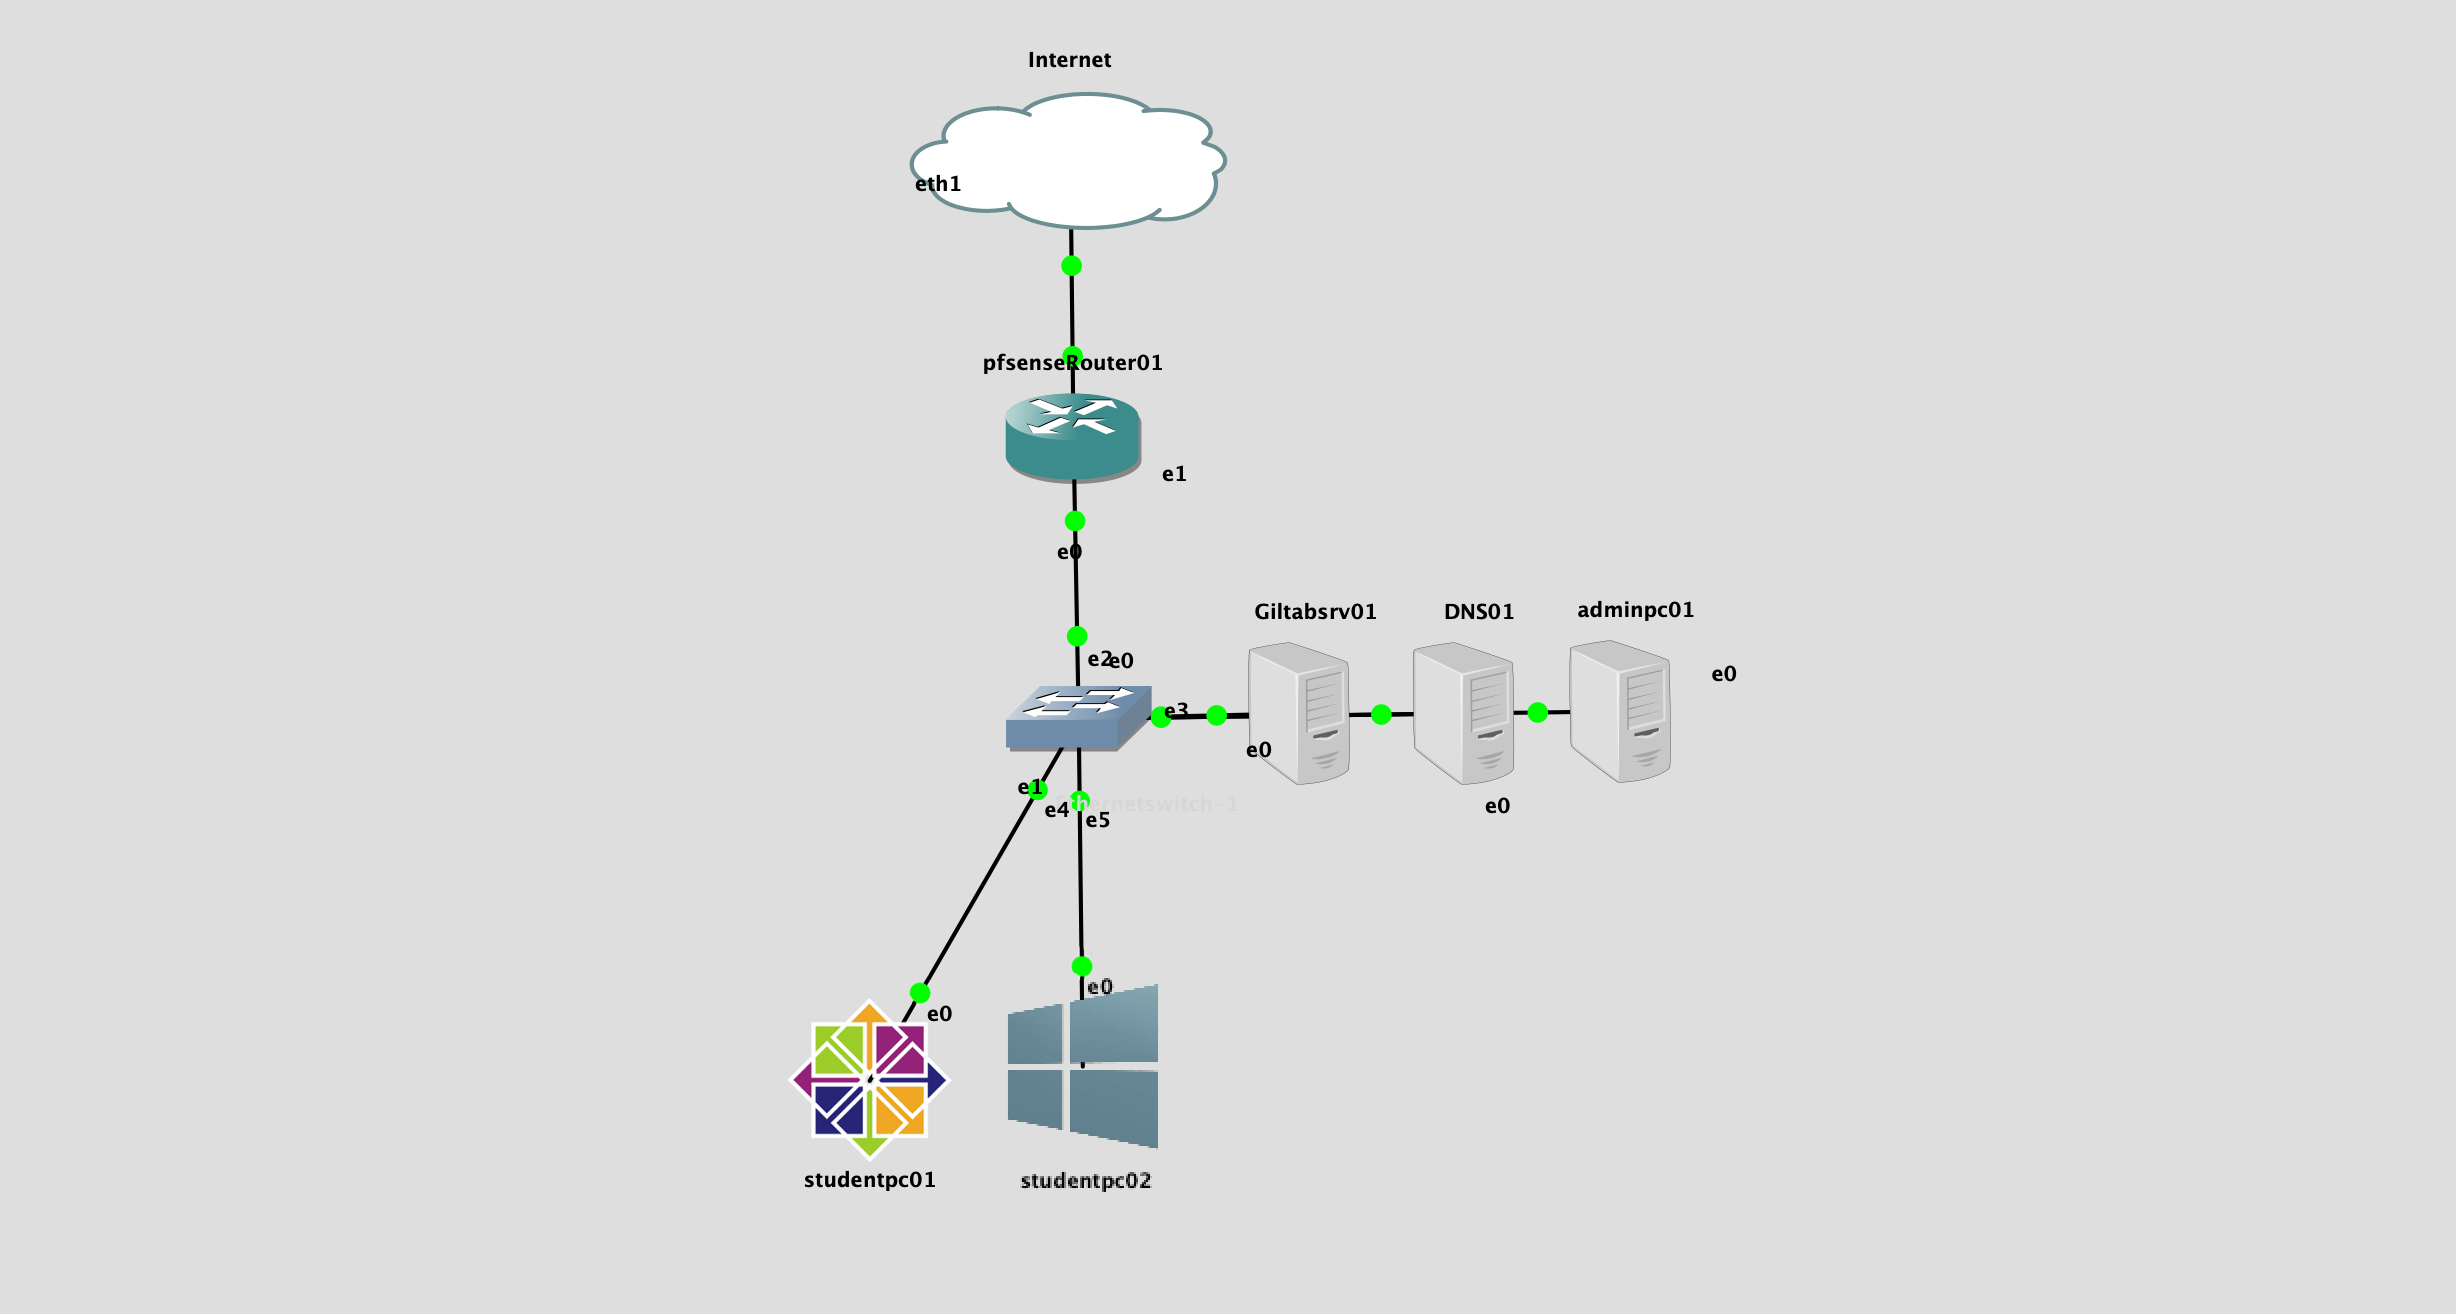
\includegraphics[width=\linewidth]{img/gns3FinalPoC.jpg}
	\caption{Opstelling voorgesteld in GNS3}
	\label{fig:PoC1}
\end{figure}

\subsection{Functionaliteiten}

Hier volgt een opsomming van alle functionaliteiten die een dergelijke opstelling bevat.

\begin{itemize}
	\item Alle admin systemen zijn gehardened en beveiligd volgens een Baseline gebaseerd op de CIS Guidelines.
	\item De het opzetten van de omgeving voor een examen wordt grotendeels door Ansible gedaan.
	\item Het is simpel om de examenomgeving op te zetten voor een lector (dankzij Ansible). 
	\item De studenten kunnen enkel browsen naar websites die toegestaan zijn door de lecoren.
	\item Beveiliging op zowel de firewall en DNS zorgen ervoor dat studenten geen VPN-verbinding kunnen maken of een andere DNS Server kunnen gebruiken.
	\item Studenten kunnen hun examen van de lokale Gitlab server halen en na het examen indienen via Gitlab
	\item Er wordt gemonitord of studenten niet met andere netwerken verbinden.
\end{itemize}

\subsection{Ontbrekende functionaliteiten}

Deze proof of concept is geen ideale oplossing voor het nieuwe examensysteem, het is wel de meest ideale oplossing binnen dit onderzoek.
Toch blijft er een functionaliteit over die voor sommige examens een nice-to-have is en voor andere een must-have, namelijk: 

Studenten hebben volledige toegang tot documenten op hun eigen laptop. Indien zij reeds gemaakte oefeningen, opgeloste voorbeeldexamens of vorige versies van examens bij zouden hebben, is het mogelijk dat zij een oneerlijk voordeel krijgen tegenover studenten die dit niet bijhebben. Volgens een lector die programmeerexamens afneemt, maakt dat voor examens zoals Object-Geori\"{e}nteerd Programmeren III minder uit vergeleken met Object-Geori\"{e}nteerd Programmeren I, waar het die lector noodzakelijk is dat studenten geen toegang hebben tot alle oefeningen, bijvoorbeeld.

\subsection{Automatisatie}
Automatisatie gebeurt met Ansible. Ansible communiceert met de servers via SSH met 4096bit SSH keys. Het is niet mogelijk om op die servers met een wachtwoord in te loggen.

\subsubsection{DNS \& Firewall}
Wanneer studenten toch websites mogen bezoeken zoals bijvoorbeeld de java api, moet er een aanpassing gemaakt worden in DNS en Firewall. Wanneer de lector de URL van een site ingeeft bij het uitvoeren van de ansible playbook, worden de juiste aanpassingen gemaakt op beide servers.

\subsection{Gitlab}
Gebruikers worden in deze proof-of-concept via de Gitlab API toegevoegd met Ansible. Wanneer de docent gebruikers aanlevert in een .csv bestand, dan leest Ansible die uit en voegt ze toe aan de Gitlab server. 

Dit is de Ansible taak die per student in die .csv file uitgevoerd wordt. De waarden die tussen: "\{\{\}\}"   staan, zijn variabelen die per student verschillend zijn.
\lstset{basicstyle=\ttfamily}
\begin{lstlisting}
-  name: Create Gitlab User
	gitlab_user:
		server_url: https://gitlabsrv01.benoitballiu.be
		validate_certs: True
		api_username: admin
		api_password: $encrypted$
		group: "{{ group }}"
		access_level: developer
		name: "{{ studentName }}"
		username: "{{ username }}"
		email: "{{ studentEmail }}"
		password: dummypassword
		state: present
	delegate_to: localhost
\end{lstlisting}

Het volledige Ansible Playbook kan u in de bijlagen terugvinden.

\section{Verloop van een examen}
Deze sectie geeft meer uitleg over BYOD-examen met deze opstelling, door een voorbeeld van het verloop te geven.

\subsection{Voorbeeld: Examen OOPII}

\begin{itemize}
	\item De lector bereidt de avond voor het examen of op de dag zelf het examen voor, door een een Ansible Playbook te doorlopen. Ansible zal zo users, studenten die het examen afleggen, toevoegen aan zowel de gitlabserver als de Captive portal van de router en, indien gewild, url's te whitelisten. Zie figuur \hyperref[fig:PoC2]{4.2}, dit is het scherm dat de lector invult. Zowel figuur \hyperref[fig:PoC3]{4.3} als figuur \hyperref[fig:PoC4]{4.4} voor een voorbeeld van de files die de lector moet invullen. 

	\begin{figure}[H]
		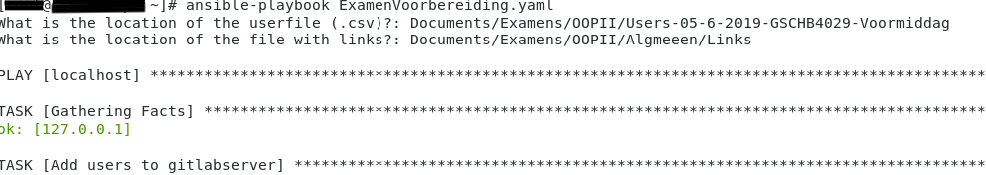
\includegraphics[width=\linewidth]{img/AdminPC.png}
		\caption[Voorbeeld van het Ansible Playbook]{Dit is hoe een docent een examen voorbereidt. een lector geeft hier de locaties van de gevraagde bestanden in.}
		\label{fig:PoC2}
	\end{figure}
	
	\begin{figure}[H]
	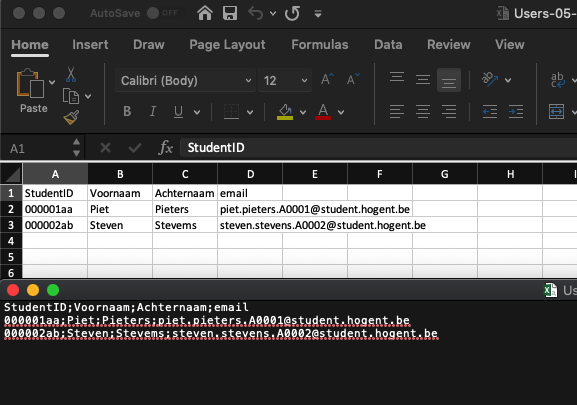
\includegraphics[width=\linewidth]{img/CSV1.png}
	\caption[Voorbeeld van Users.csv]{Boven zie je een voorbeeld van een User file die een lector invult, onder zie je dezelfde file op de manier dat Ansible hem inleest.}
	\label{fig:PoC3}
\end{figure}

	\begin{figure}[H]
	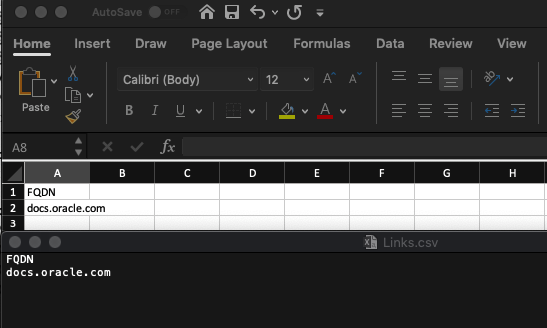
\includegraphics[width=\linewidth]{img/CSV2.png}
	\caption[Voorbeeld van Links.csv] {Boven zie je een voorbeeld van een Link file die een lector invult, onder zie je dezelfde file op de manier dat Ansible hem inleest.}
	\label{fig:PoC4}
\end{figure}

	\item De lector kan op de adminmachine testen of de studenten enkel aan de toegestane url's kunnen.
	
		\begin{figure}[H]
		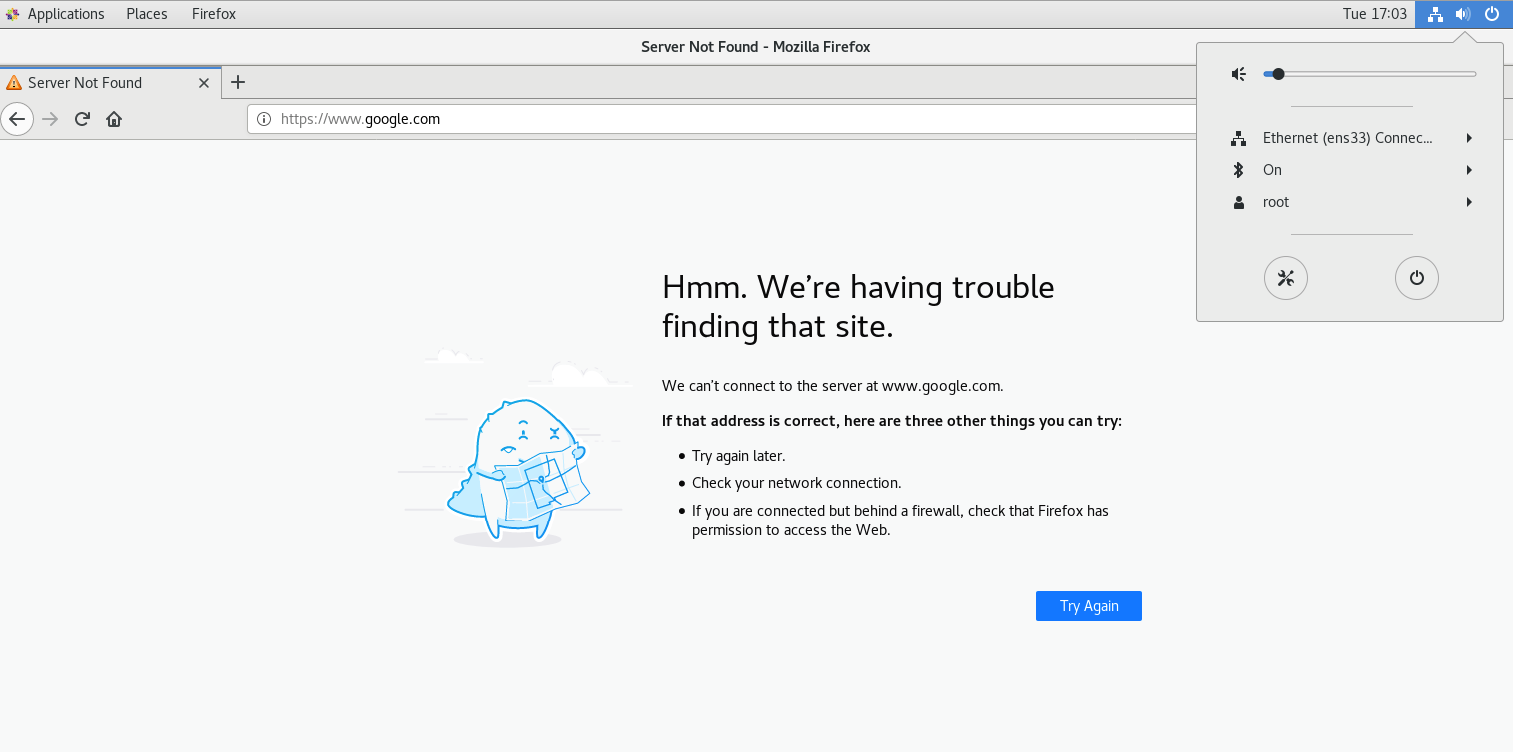
\includegraphics[width=\linewidth]{img/Linkblock1.png}
		\caption[Screenshot van webbrowser 1] {Hierboven zie je een screenshot van wat er gebeurt wanneer de docent een site verschillend van de toegelaten sites uittest.}
		\label{fig:PoC5}
	\end{figure}

		\begin{figure}[H]
		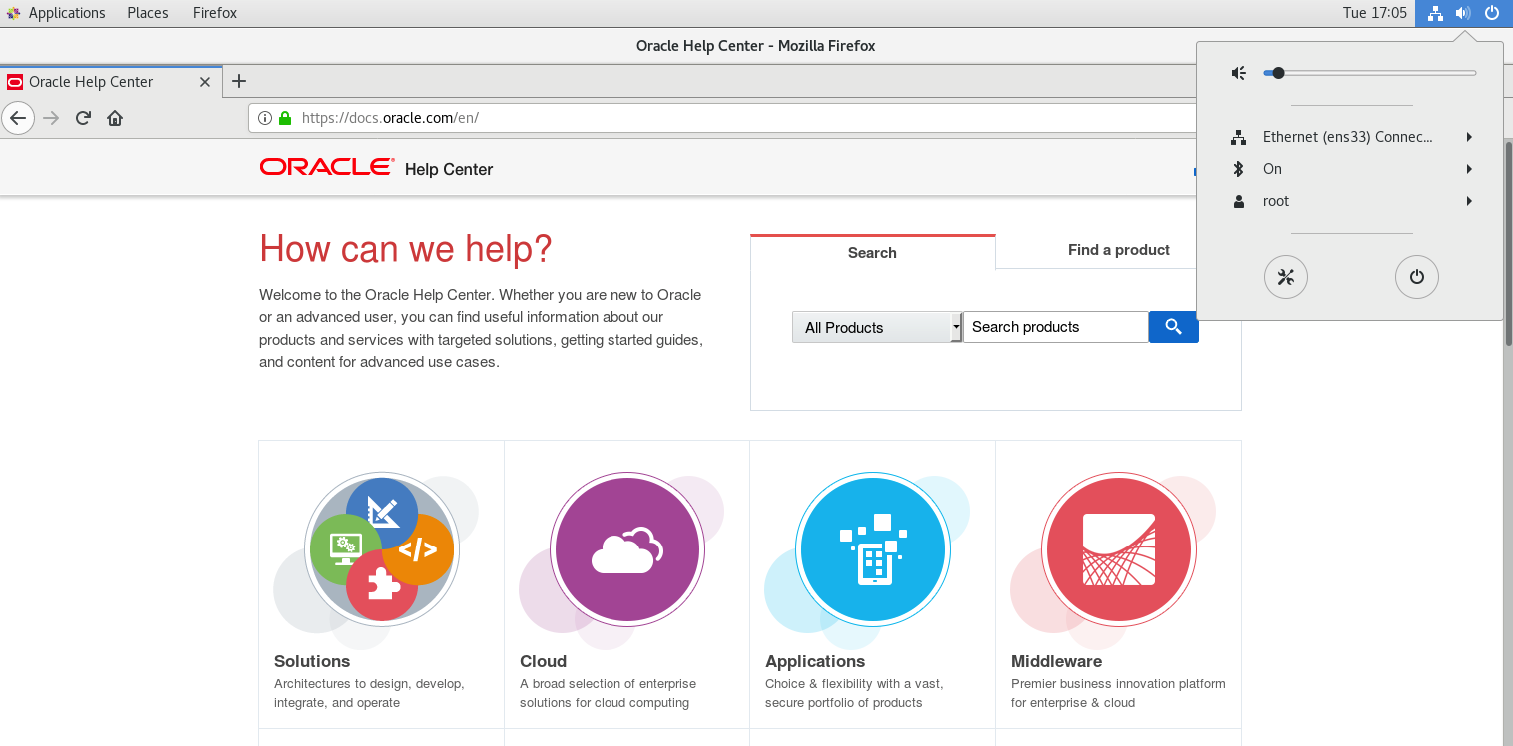
\includegraphics[width=\linewidth]{img/Linkblock2.png}
		\caption[Screenshot van webbrowser 2] {Hierboven zie je een screenshot van wat er gebeurt wanneer de docent één van de toegestane sites uittest.}
		\label{fig:PoC6}
	\end{figure}
	\item De lector voegt zijn project toe aan Gitlab. Dit kan hij manueel doen: 
			\begin{figure}[H]
		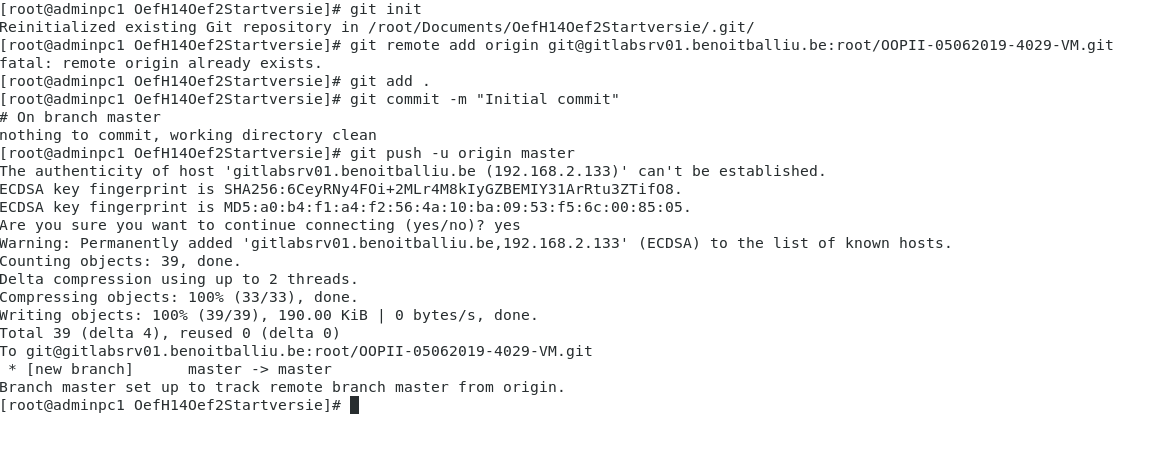
\includegraphics[width=\linewidth]{img/Git01.png}
		\caption[Screenshot van het aanmaken van een git repository] {Hierboven zie je een screenshot waar een lector een nieuw repository toegvoegt aan de gitlabserver.}
		\label{fig:PoC7}
	\end{figure}
    Gezien het thema van automatisatie is dit in het eindelijke playbook toch geautomatiseerd. 
   			\begin{figure}[H]
   	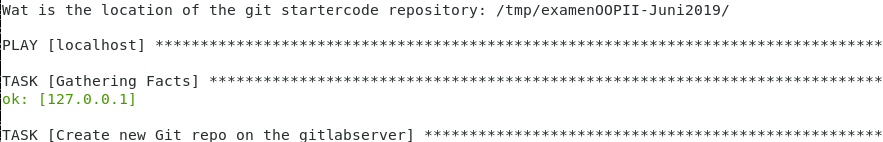
\includegraphics[width=\linewidth]{img/Git02.png}
   	\caption[Screenshot van het aanamken van een git repository met Ansible] {Hierboven zie je hoe het aanmaken van een gitlabproces geautomatiseerd is.}
   	\label{fig:PoC8}
   \end{figure} 
	\item Wanneer de studenten binnenkomen forken ze hun eigen private repository van het examenproject.
	
	   			\begin{figure}[H]
		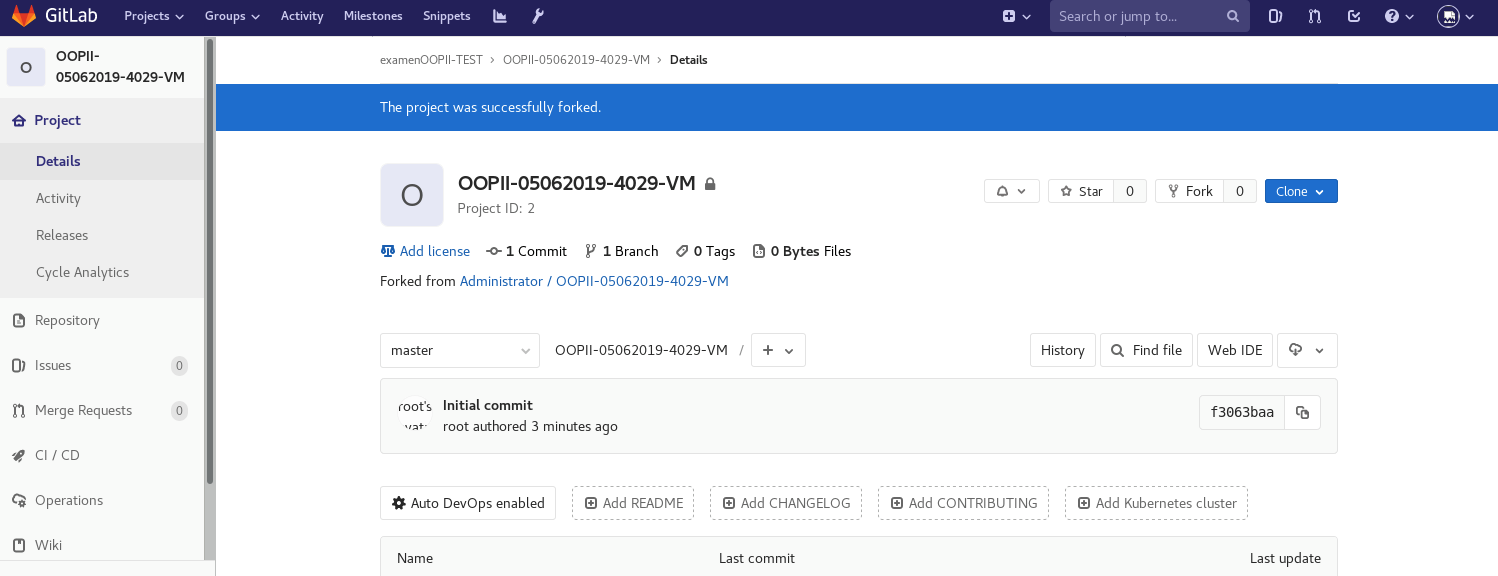
\includegraphics[width=\linewidth]{img/Fork1.png}
		\caption[Screenshot van een forked repository] {Hierboven zie je hoe de student een fork van de starterscode kan maken.}
		\label{fig:PoC9}
	\end{figure} 
	
	\item Tijdens het examen kunnen de studenten reeds pushen naar hun repository. Op het einde van het examen controleert de student of zijn oplossing correct op github staat.
	\item De Lector kan nu alle repositories van de studenten binnenhalen en verbeteren.
	   			\begin{figure}[H]
		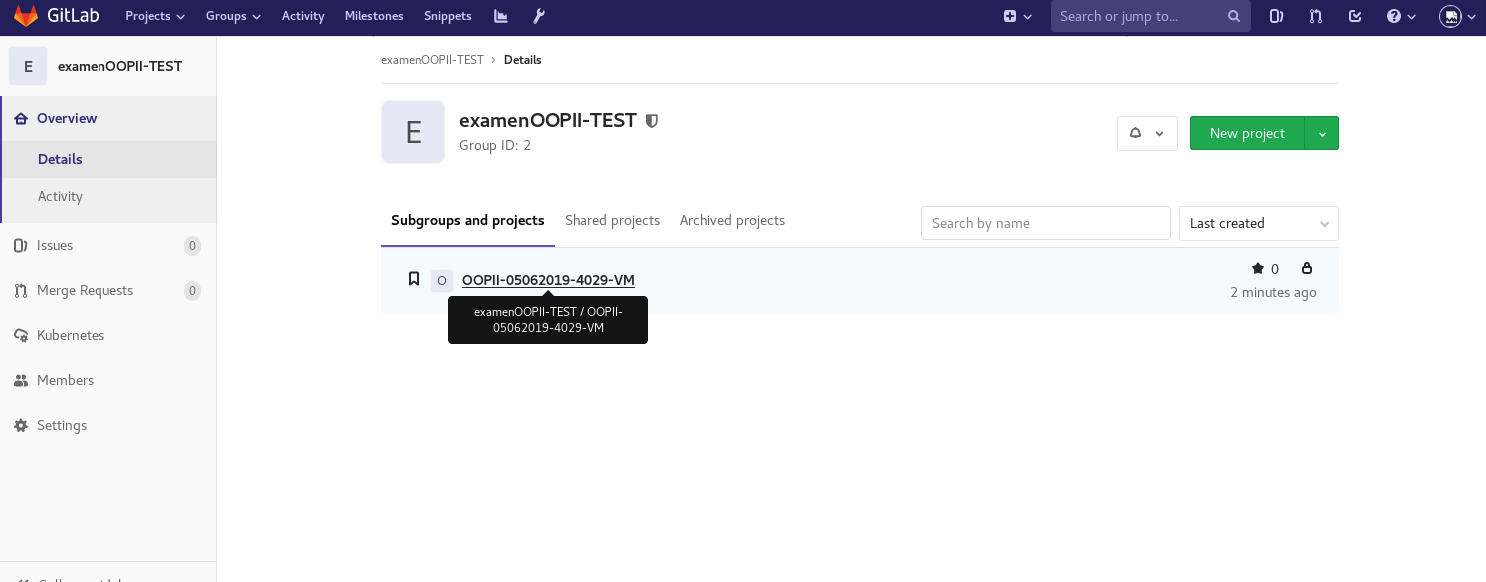
\includegraphics[width=\linewidth]{img/Check01.png}
		\caption[Screenshot van het overzicht die een lector heeft.] {Hierboven zie je wat de lector ziet na een examen, in dit geval heeft slechts 1 student een fork gemaakt}
		\label{fig:PoC10}
	\end{figure} 
	
	
\end{itemize}




